%!TEX root = popl2018.tex


\section{Decision procedure for $\strline[\replaceall]$: The single-letter case} \label{sec:replaceallsl}





%%%%%%%%%%%%%%%%%%%%%%%%%%%%%%%%%
%%%%%%%%%%%%%%%%%%%%%%%%%%%%%%%%%
\hide{
\subsection{Encode concatenation by replaceall}

We will transform a given constraint $\varphi$ into a constraint $\varphi'$ which is concatenation free. As the first step, we extend the original alphabet with two fresh letters $a,b$.

For each $x=yz$, we introduce a new variable $x'$ and replace $x=yz$ by two new constraints
$x'=\replaceall(ab, a, x)$ and $x=\replaceall(x', b, z)$.

\begin{proposition}
	$\varphi$ and $\varphi'$ are equisatisfiable.
\end{proposition}
}
%%%%%%%%%%%%%%%%%%%%%%%%%%%%%%%%%
%%%%%%%%%%%%%%%%%%%%%%%%%%%%%%%%%


%\subsection{The single-letter case}

In this section, we consider the single-letter case, that is, for the $\strline[\replaceall]$ formula $C = \varphi \wedge \psi$, every term of the form $\replaceall(z, e, z')$ in $\varphi$ satisfies that $e=a$ for $a \in \Sigma$.
We begin by explaining the idea of the decision procedure in the case where there is a single use of a $\replaceall(\cdots)$ term.
Then we describe the decision procedure in full details.

%We first assume that the regular constraint $\psi = \bigwedge \limits_{x \in \vars(\varphi)} x \in e_x$, that is, there is exactly one atomic regular constraint for each variable.

%We first explain the basic idea of the decision procedure.

\subsection{A single use of $\replaceall(\cdots)$}

Let us start with the simple case that
\[C \equiv x = \replaceall(y, a, z) \wedge x \in e_1 \wedge y \in e_2 \wedge z \in e_3,\]
where, for $i =1, 2, 3$, we suppose  $\cA_i = (Q_i, \delta_i, q_{0,i}, F_i)$
%\cA_y = (Q_y, \delta_y, q_{0, y}, F_y), \cA_z = (Q_z, \delta_z, q_{0, z}, F_z)$
is the NFA corresponding to the regular expression $e_i$.

From the semantics, $C$ is satisfiable if and only if $x, y, z$ can be assigned with strings $u, v, w$ so that: (1) $u$ is obtained from $v$ by replacing all the occurrences of $a$ in $v$ with $w$, and (2) $u, v, w$ are accepted by $\cA_1, \cA_2, \cA_3$ respectively. Let $u,v,w$ be the strings satisfying these two constraints. As $u$ is accepted by $\cA_1$,  there must be an accepting run of $\cA_1$ on $u$. Let $v = v_1 a v_2 a \cdots a v_k$ such that for each $i \in [k]$, $v_i \in (\Sigma \setminus \{a\})^*$. Then $u = v_1 w v_2 w \cdots w v_k$ and there are states $q_1, q'_1, \cdots, q_{k-1}, q'_{k-1}, q_k$  such that
%
$$
q_{0,1} \xrightarrow[\cA_1]{v_1} q_1 \xrightarrow[\cA_1]{w} q'_1 \xrightarrow[\cA_1]{v_2} q_2 \xrightarrow[\cA_1]{w} q'_2 \cdots q_{k-1} \xrightarrow[\cA_1]{w} q'_{k-1} \xrightarrow[\cA_1]{v_k} q_k
$$
%
 and $q_k \in F_{1}$. Let $T_z$ denote $\left\{(q_i, q'_i) \mid i \in [k-1] \right\}$. Then $w \in \Ll(\cA_3)\ \cap\ \bigcap \limits_{(q, q') \in T_z} \Ll(\cA_1(q, q'))$. In addition, let  $\cB_{\cA_1,a,T_z}$ be the NFA obtained from $\cA_1$ by removing all the $a$-transitions first and then adding the $a$-transitions $(q, a, q')$ for $(q, q') \in T_z$. Then
 %
$$
q_{0,1} \xrightarrow[\cB_{\cA_1,a,T_z}]{v_1} q_1 \xrightarrow[\cB_{\cA_1,a,T_z}]{a} q'_1 \xrightarrow[\cB_{\cA_1,a,T_z}]{v_2} q_2 \xrightarrow[\cB_{\cA_1,a,T_z}]{a} q'_2 \cdots q_{k-1} \xrightarrow[\cB_{\cA_1,a,T_z}]{a} q'_{k-1} \xrightarrow[\cB_{\cA_1,a,T_z}]{v_k} q_k.
$$
%
Therefore,
$v \in \Ll(\cA_2) \cap \Ll(\cB_{\cA_1,a,T_z})$. We deduce that there is $T_z \subseteq Q_1 \times Q_1$ such that $\Ll(\cA_3)\ \cap\ \bigcap \limits_{(q, q') \in T_z} \Ll(\cA_1(q, q')) \neq \emptyset$ and $ \Ll(\cA_2) \cap \Ll(\cB_{\cA_1,a,T_z}) \neq \emptyset$. In addition, it is not hard to see that this condition is also sufficient for the satisfiability of $C$. The arguments proceed as follows: Let $v \in  \Ll(\cA_2) \cap \Ll(\cB_{\cA_1,a,T_z})$ and $w \in \Ll(\cA_3)\ \cap\ \bigcap \limits_{(q, q') \in T_z} \Ll(\cA_1(q, q'))$. From $v \in \Ll(\cB_{\cA_1,a,T_z})$, we know that there is an accepting run of $\cB_{\cA_1,a,T_z}$ on $v$. Recall that $\cB_{\cA_1,a,T_z}$ is obtained from $\cA_1$ by first removing all the $a$-transitions, then adding all the transitions $(q,a,q')$ for $(q,q') \in T_z$.  Suppose $v = v_1 a v_2 \cdots a v_k$ such that $v_i \in (\Sigma \setminus \{a\})^*$ for each $i \in [k]$ and
$$
q_{0,1} \xrightarrow[\cB_{\cA_1,a,T_z}]{v_1} q_1 \xrightarrow[\cB_{\cA_1,a,T_z}]{a} q'_1 \xrightarrow[\cB_{\cA_1,a,T_z}]{v_2} q_2 \xrightarrow[\cB_{\cA_1,a,T_z}]{a} q'_2 \cdots q_{k-1} \xrightarrow[\cB_{\cA_1,a,T_z}]{a} q'_{k-1} \xrightarrow[\cB_{\cA_1,a,T_z}]{v_k} q_k
$$
is an accepting run of $\cB_{\cA_1,a,T_z}$ on $v$. Then $q_{0,1} \xrightarrow[\cA_1]{v_1} q_1$, and for each $i \in [k-1]$ we have $(q_i, q'_i) \in T_z$ and $q'_i \xrightarrow[\cA_1]{v_{i+1}} q'_{i+1}$; moreover, $q_k \in F_1$.
Let $u = \replaceall(v, a, w)=v_1 w v_2 \cdots w v_k$. Since $w \in \bigcap \limits_{(q, q') \in T_z} \Ll(\cA_1(q, q'))$,  we infer that
$$
q_{0,1} \xrightarrow[\cA_1]{v_1} q_1 \xrightarrow[\cA_1]{w} q'_1 \xrightarrow[\cA_1]{v_2} q_2 \xrightarrow[\cA_1]{w} q'_2 \cdots q_{k-1} \xrightarrow[\cA_1]{w} q'_{k-1} \xrightarrow[\cA_1]{v_k} q_k
$$
is an accepting run of $\cA_1$ on $u$. Therefore, $u$ is accepted by $\cA_1$ and $C$ is satisfiable.

\begin{proposition}\label{prop-sat-sl-case}
Let $C \equiv x = \replaceall(y, a, z) \wedge x \in e_1 \wedge y \in e_2 \wedge z \in e_3$. Then $C$ is satisfiable iff there is a set $T_{z} \subseteq Q_1 \times Q_1$ such that $\Ll(\cA_3)\ \cap\ \bigcap \limits_{(q, q') \in T_z} \Ll(\cA_1(q, q')) \neq \emptyset$ and $ \Ll(\cA_2) \cap \Ll(\cB_{\cA_1,a,T_z}) \neq \emptyset$.
\end{proposition}

From Proposition~\ref{prop-sat-sl-case}, we can decide the satisfiability of $C$ in polynomial space as follows:
\begin{description}
\item[Step I.] Guess a set $T_{z} \subseteq Q_1 \times Q_1$.
%
\item[Step II.] Guess an accepting run of the product automaton of $\cA_3$ and $\cA_1(q, q')$ for $(q,q') \in T_{z}$.
%
\item[Step III.] Guess an accepting run of the product automaton of $\cA_2$ and $\cB_{\cA_1, a,  T_{z}}$.
\end{description}
During Step II and III, it is sufficient to record $T_z$ and a state of the product automaton, which occupies only a polynomial space.

The above decision procedure can be easily generalised to the case that there are multiple atomic regular constraints for $x$. For instance, let $x \in e_{1,1} \wedge x \in e_{1,2}$ and for $j = 1, 2$, $\cA_{1,j} = (Q_{1,j}, \delta_{1, j}, q_{0,1, j}, F_{1,j})$ be
the NFA corresponding to $e_{1,j}$. Then in Step I, two sets $T_{1,z} \subseteq Q_{1,1} \times Q_{1,1}$ and $T_{2,z} \subseteq Q_{1,2} \times Q_{1,2}$ are guessed, moreover, Step II and III are adjusted accordingly.

\begin{example}\label{exmp-sl}
Let $C \equiv x= \replaceall(y, 0, z) \wedge x \in e_1 \wedge y \in e_2 \wedge z \in e_3$, where $e_1=(0+1)^* (00(0+1)^* + 11(0+1)^*)$,  $e_2= (01)^*$,  and $e_3 = (10)^*$. The NFA $\cA_{1}, \cA_{2}, \cA_{3}$ corresponding to $e_1, e_2, e_3$ respectively are illustrated in Figure~\ref{fig-sl-exmp}. Let $T_z = \{(q_0, q_0), (q_1, q_2)\}$.  Then
$$
\begin{array}{l c l}
 \Ll(\cA_3)\ \cap\ \bigcap \limits_{(q, q') \in T_z} \Ll(\cA_1(q, q'))  & = & \Ll(\cA_3)\ \cap \Ll(\cA_1(q_0, q_0)) \cap \Ll(\cA_1(q_1,q_2)) \\
& = & \Ll((10)^*) \cap \Ll((0+1)^*) \cap \Ll(1(0+1)^*) \\
& \neq & \emptyset.
\end{array}
$$
In addition, $\cB_{\cA_1, 0, T_z}$ (also illustrated in Figure~\ref{fig-sl-exmp}) is obtained from $\cA_1$ by removing all the $0$-transitions, then adding the transitions $(q_0, 0, q_0)$ and $(q_1, 0, q_2)$. Then
$$
 \Ll(\cA_2) \cap \Ll(\cB_{\cA_1,0,T_z})   =  \Ll((01)^*) \cap \Ll((0+1)^* 10 1^*) \neq \emptyset.
$$
Therefore, we can choose $z$ to be a string from $\Ll(\cA_3) \cap \ \bigcap \limits_{(q, q') \in T_z} \Ll(\cA_1(q, q'))=\Ll((10)^*) \cap \Ll((0+1)^*) \cap \Ll(1(0+1)^*)$, say $10$, and $y$ to be a string from $ \Ll(\cA_2) \cap \Ll(\cB_{\cA_1,0,T_z})   =  \Ll((01)^*) \cap \Ll((0+1)^* 10 1^*)$, say $0101$,  then $x$ gets the value $\replaceall(0101, 0, 10)=101101$, which is in $\Ll(\cA_1)$. Therefore, $C$ is satisfiable.\qed
%
\begin{figure}[htbp]
\begin{center}
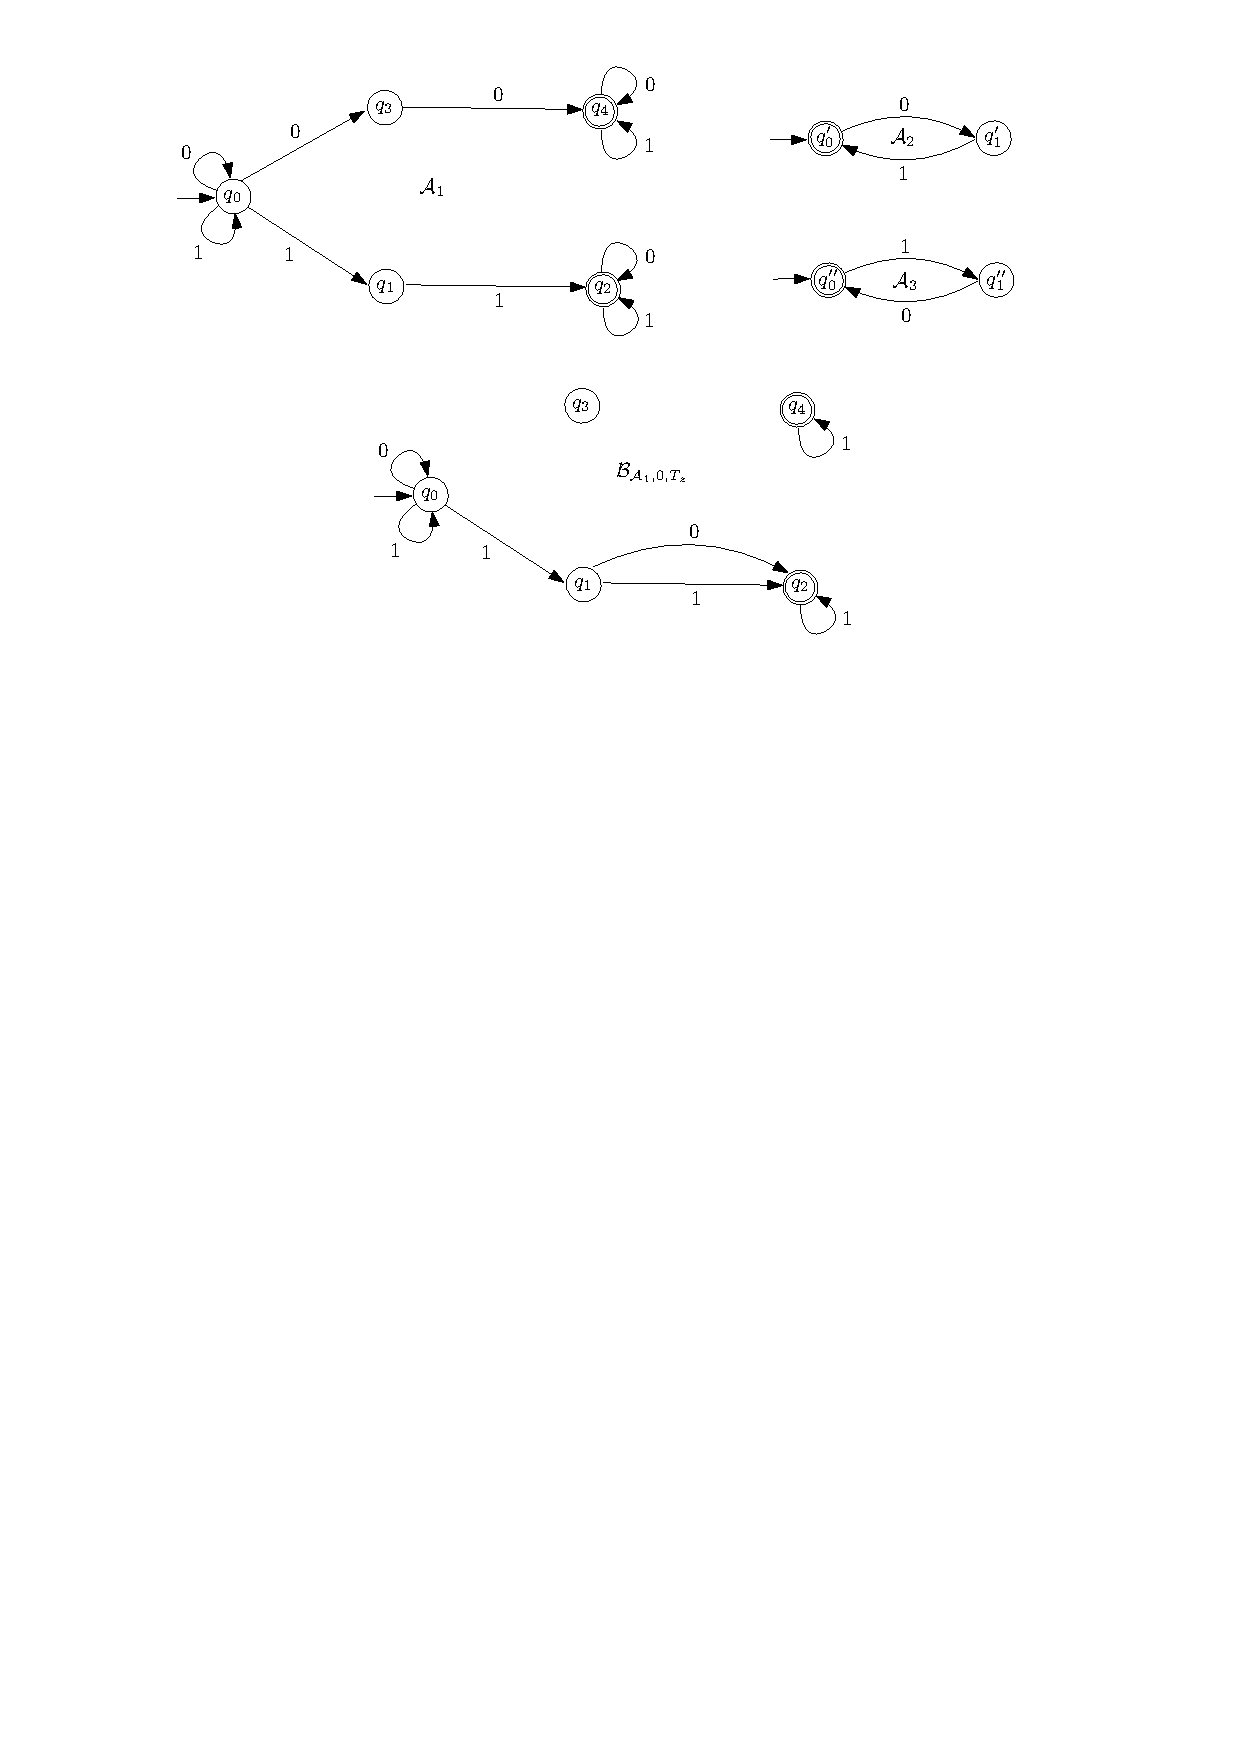
\includegraphics[scale=0.65]{single-letter-example.pdf}
\end{center}
\caption{An example for the single-letter case: One $\replaceall$}\label{fig-sl-exmp}
\end{figure}
\end{example}


\subsection{The general case}

Let us now consider the general case where $C$ contains multiple occurrences of $\replaceall(\cdots)$ terms.
Then the satisfiability of $C$ is decided by the following two-step procedure.

\smallskip

\noindent{\bf Step I.} We utilise the dependency graph $C$ and compute nondeterministically a collection of atomic regular constraints $\cE(x)$ for each variable $x$, in a top-down manner.

%During the computation, for each variable $x$, the collection of atomic regular constraints
Notice that $\cE(x)$ is represented succinctly as a set of pairs $(\cT, \cP)$, where $\cT=(Q, \delta)$ is a transition graph and $\cP \subseteq Q \times Q$. The intention of $(\cT, \cP)$ is to represent succinctly the collection of the atomic regular constraints containing $(Q, \delta, q, \{q'\})$ for each $(q,q') \in \cP$, where $q$ is the initial state and $\{q'\}$ is the set of final states.

%\tl{you want to say that all regular constraints $\cE(x)$ share the same "underlying" graph, but differ in the initial and final states.} \tl{I rephrased a bit-- the original was commented below. Check whether this is what you mean}

Initially, let $G_0:= G_C$.  In addition, for each variable $x$ with the conjunct $x \in e$ in $\psi$ we define $\cE_0(x)$ as follows.  Let $\cA=(Q, \delta, q_0, F)$ be the NFA corresponding to $e$. We nondeterministically choose $q \in F$ and set $\cE_0(x):=  \{((Q, \delta), \{(q_0, q)\})\}$.


%In addition, for each variable $x$, compute $\cE_0(x)$ as follows: Initially, let $\cE_0(x) := \emptyset$.
%For each conjunct $x \in e$ in $\psi$, let $\cA=(Q, \delta, q_0, F)$ be the NFA corresponding to $e$, then nondeterministically choose $q \in F$ and let $\cE_0(x):= \cE_0(x) \cup \{((Q, \delta), \{(q_0, q)\})\}$.
%

We begin with $i:= 0$ and repeat the following procedure until we reach some $i$ where $G_i$ is an empty graph, i.e. a graph without edges.
Note that $G_0$ was defined above.
\begin{enumerate}
\item Select a vertex $x$ of $G_i$ such that $x$ has no predecessors  and has two successors in $G_i$. Suppose $(x, (\rpleft, a), y)$ and $(x, (\rpright,a), z)$ are the two edges out of $x$ in $G_i$ and $\cE_i(x)=\{(\cT_1,\cP_1), \cdots, (\cT_k, \cP_k)\}$, where for each $j \in [k]$, $\cT_j = (Q_j, \delta_j)$. Then $\cE_{i+1}(z)$ and  $\cE_{i+1}(y)$ and $G_{i+1}$ are computed as follows:
\begin{enumerate}
\item For each $j \in [k]$, guess a set $T_{j, z} \subseteq Q_j \times Q_j$.
%
\item If $y \neq z$, then let
$$\cE_{i+1}(z):= \cE_{i}(z) \cup \left\{(\cT_j, T_{j,z}) \mid j \in [k] \right\}$$
and
$$\cE_{i+1}(y): = \cE_{i}(y) \cup \left\{(\cT_{\cT_j, a, T_{j,z}}, \cP_j) \mid j \in [k] \right\},$$
where $\cT_{\cT_j, a, T_{j,z}}$ is obtained from $\cT_j$ by first removing all the $a$-transitions, then adding all the transitions $(q, a, q')$ for $(q,q') \in T_{j,z}$.

Otherwise, let
$$\cE_{i+1}(z):= \cE_{i}(z) \cup \left\{(\cT_j, T_{j,z}) \mid j \in [k] \right\} \cup \left\{(\cT_{\cT_j, a, T_{j,z}}, \cP_j) \mid j \in [k] \right\}.$$
In addition, for each vertex $x'$ distinct from $x, y, z$, let $\cE_{i+1}(x') := \cE_i(x')$.
We set $\cE_{i+1}(x) = \emptyset$.
%
\item Let $G_{i+1}:= G_i \setminus \{(x, (\rpleft, a), y), (x, (\rpright,a), z)\}$.
\end{enumerate}
%
\item Let $i: = i+1$.
\end{enumerate}

For each variable $x$, let $\cE(x)$ denote the set $\cE_i(x)$ after exiting the above loop.

\smallskip

\noindent {\bf Step II.}
For each source variable $x$, guess an accepting run of the product automaton of all the NFA in $\cE(x)$.

\smallskip

%Note that in the first sight, the cardinalities of the sets $\cE(x)$ seem exponential w.r.t. the size of $C$ in the worst case and the nondeterministic algorithm may take exponential space.
%By a refined analysis, we can see that the cardinalities of the sets $\cE(x)$ are in fact polynomial.

It remains to argue the correctness and complexity of the above procedure.
Correctness follows a similar argument to Proposition~\ref{prop-sat-sl-case} and is presented at the end of this section.
We first give an example then argue the complexity.

\begin{example}
Suppose $C \equiv x= \replaceall(y, 0, z) \wedge y = \replaceall(y', 1, z') \wedge x \in e_1 \wedge y \in e_2 \wedge z \in e_3 \wedge y' \in e_4  \wedge z' \in e_5$, where $e_1, e_2, e_3$ are as in Example~\ref{exmp-sl}, $e_4=0^* 1^* 0^* 1^*$, and $e_5=0^*1^*$. Let $\cA_4,\cA_5$ be the NFA corresponding to $e_4$ and $e_5$ respectively (see Figure~\ref{fig-sl-exmp-nested}). The dependency graph $G_C$ of $C$ is illustrated in Figure~\ref{fig-sl-exmp-nested}. Let $\cT_1,\cdots, \cT_5$ be the transition graph of $\cA_1,\cdots, \cA_5$ respectively. Then the collection of regular constraints $\cE(\cdot)$ are computed as follows.
\begin{itemize}
\item Let $G_0=G_C$. We nondeterministically choose $\cE_0(x) = \{(\cT_1, \{(q_0, q_2)\})\}$, $\cE_0(y) = \{(\cT_2, \{(q^\prime_0, q^\prime_0)\})\}$, $\cE_0(z) = \{(\cT_3, \{(q^{\prime\prime}_0, q^{\prime\prime}_0)\})\}$, $\cE_0(y^\prime) = \{(\cT_4, \{(p_0, p_1)\})\}$, $\cE_0(z^\prime) = \{(\cT_5, \{(p^{\prime}_0, p^{\prime}_1)\})\}$.
%
\item Select the vertex $x$ in $G_0$, construct $\cE_1(y)$ and $\cE_1(z)$ as in Example~\ref{exmp-sl}, that is, nondeterministically choose $T_z =\{(q_0, q_0), (q_1,q_2)\}$, let $\cE_1(z) = \{(\cT_3, \{(q^{\prime\prime}_0, q^{\prime\prime}_0)\}), (\cT_1, \{(q_0,q_0), (q_1, q_2)\})\}$ and $\cE_1(y)=\{(\cT_2, \{(q^\prime_0, q^\prime_0)\}), (\cT_{\cT_1, 0, T_z}, \{(q_0,q_2)\})\}$, where $\cT_{\cT_1, 0, T_z}$ is the transition graph of $\cB_{\cA_1, 0, T_z}$ illustrated in Figure~\ref{fig-sl-exmp}. In addition, $\cE_1(x)=\cE_0(x)$, $\cE_1(y')=\cE_0(y')$ and $\cE_1(z')=\cE_0(z')$. Finally, $G_1$ is obtained from $G_0$ by removing the two edges out of $x$.
%
\item Select the vertex $y$ in $G_1$, construct $\cE_2(y')$ and $\cE_2(z')$ as follows: Nondeterministically choose $T_{1,z'} = \{(q^\prime_0, q^\prime_0)\}$  for $\cT_2$ and $T_{2,z'}=\{(q_0,q_1),(q_1,q_2)\}$ for $\cT_{\cT_1, 0, T_z}$, let
$$\cE_2(z')=\left\{(\cT_5, \{(p^{\prime}_0, p^{\prime}_1)\}), (\cT_2, \{(q^\prime_0, q^\prime_0)\}), (\cT_{\cT_1, 0, T_z}, \{(q_0,q_1),(q_1,q_2)\}) \right\},$$
and
$$\cE_2(y')=\left\{ (\cT_4, \{(p_0, p_1)\}), (\cT_{\cT_2, 1, T_{1,z'}}, \{(q^\prime_0, q^\prime_0)\}), (\cT_{\cT_{\cT_1, 0, T_z}, 1, T_{2,z'}}, \{(q_0,q_2)\}) \right\},$$
where $\cT_{\cT_2, 1, T_{1,z'}}$ and $\cT_{\cT_{\cT_1, 0, T_z}, 1, T_{2,z'}}$ are illustrated in Figure~\ref{fig-sl-exmp-nested-2}. In addition, $\cE_2(x)=\cE_1(x)$, $\cE_2(y)=\cE_1(y)$, and $\cE_2(z)=\cE_1(z)$. Finally, $G_2$ is obtained from $G_1$ by removing the two edges out of $y$.
%
\end{itemize}
Since $G_2$ contains no edges, we have $\cE(x)=\cE_2(x)$, similarly for $\cE(y)$, $\cE(z)$, $\cE(y')$, and $\cE(z')$.
For the three source variables $y', z', z$, it is not hard to check that $01$ belongs to the intersection of the regular constraints in $\cE(z')$, $11$ belongs to the intersection of the regular constraints in $\cE(y')$, and $10$ belongs to the intersection of the regular constraints in $\cE(z)$. Then $y$ takes the value $\replaceall(11, 1, 01)=0101 \in \Ll(e_2)$, and $x$ takes the value $\replaceall(0101, 0, 10)=101101 \in \Ll(e_1)$. Therefore, $C$ is satisfiable. \qed
\begin{figure}[htbp]
\begin{center}
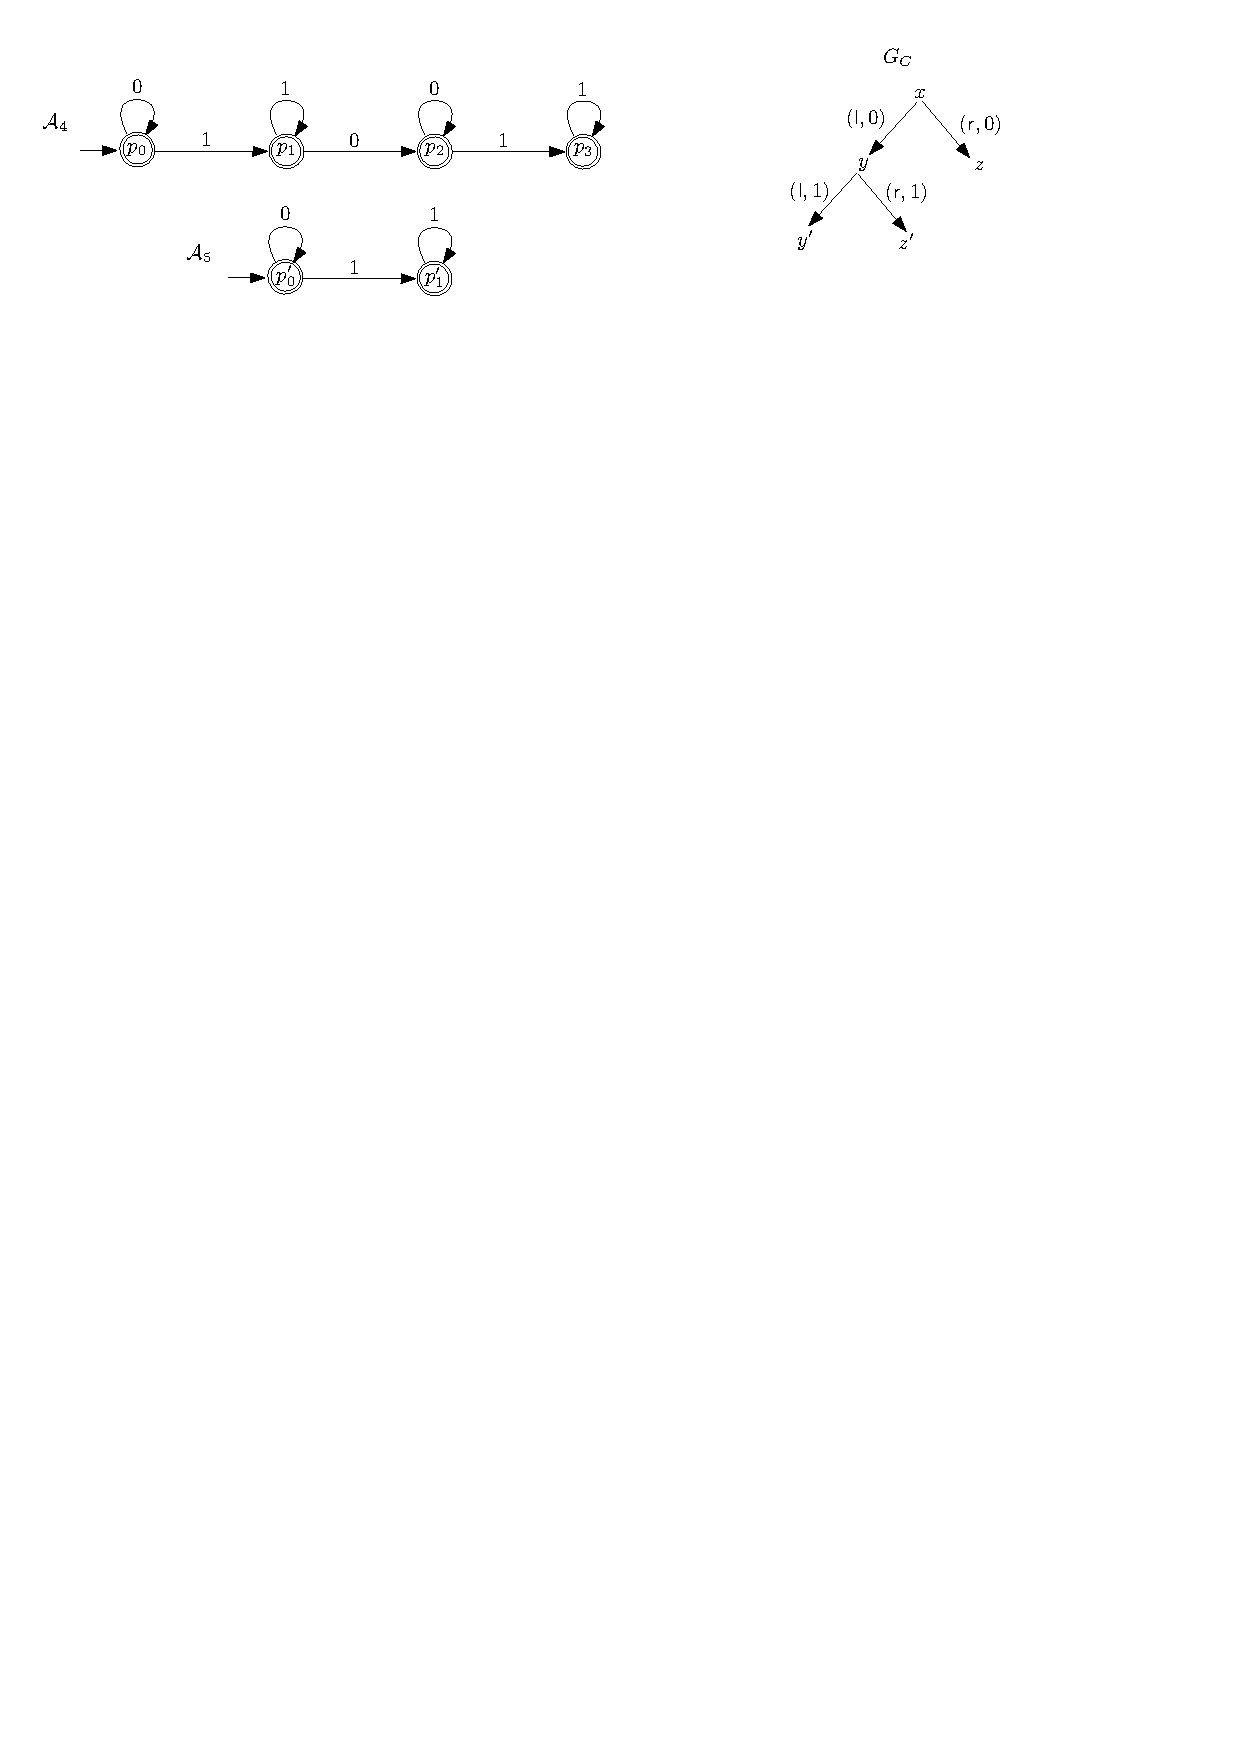
\includegraphics[scale=0.7]{single-letter-example-nested.pdf}
\end{center}
\caption{An example for the single-letter case: Multiple $\replaceall$}\label{fig-sl-exmp-nested}
\end{figure}

\begin{figure}[htbp]
\begin{center}
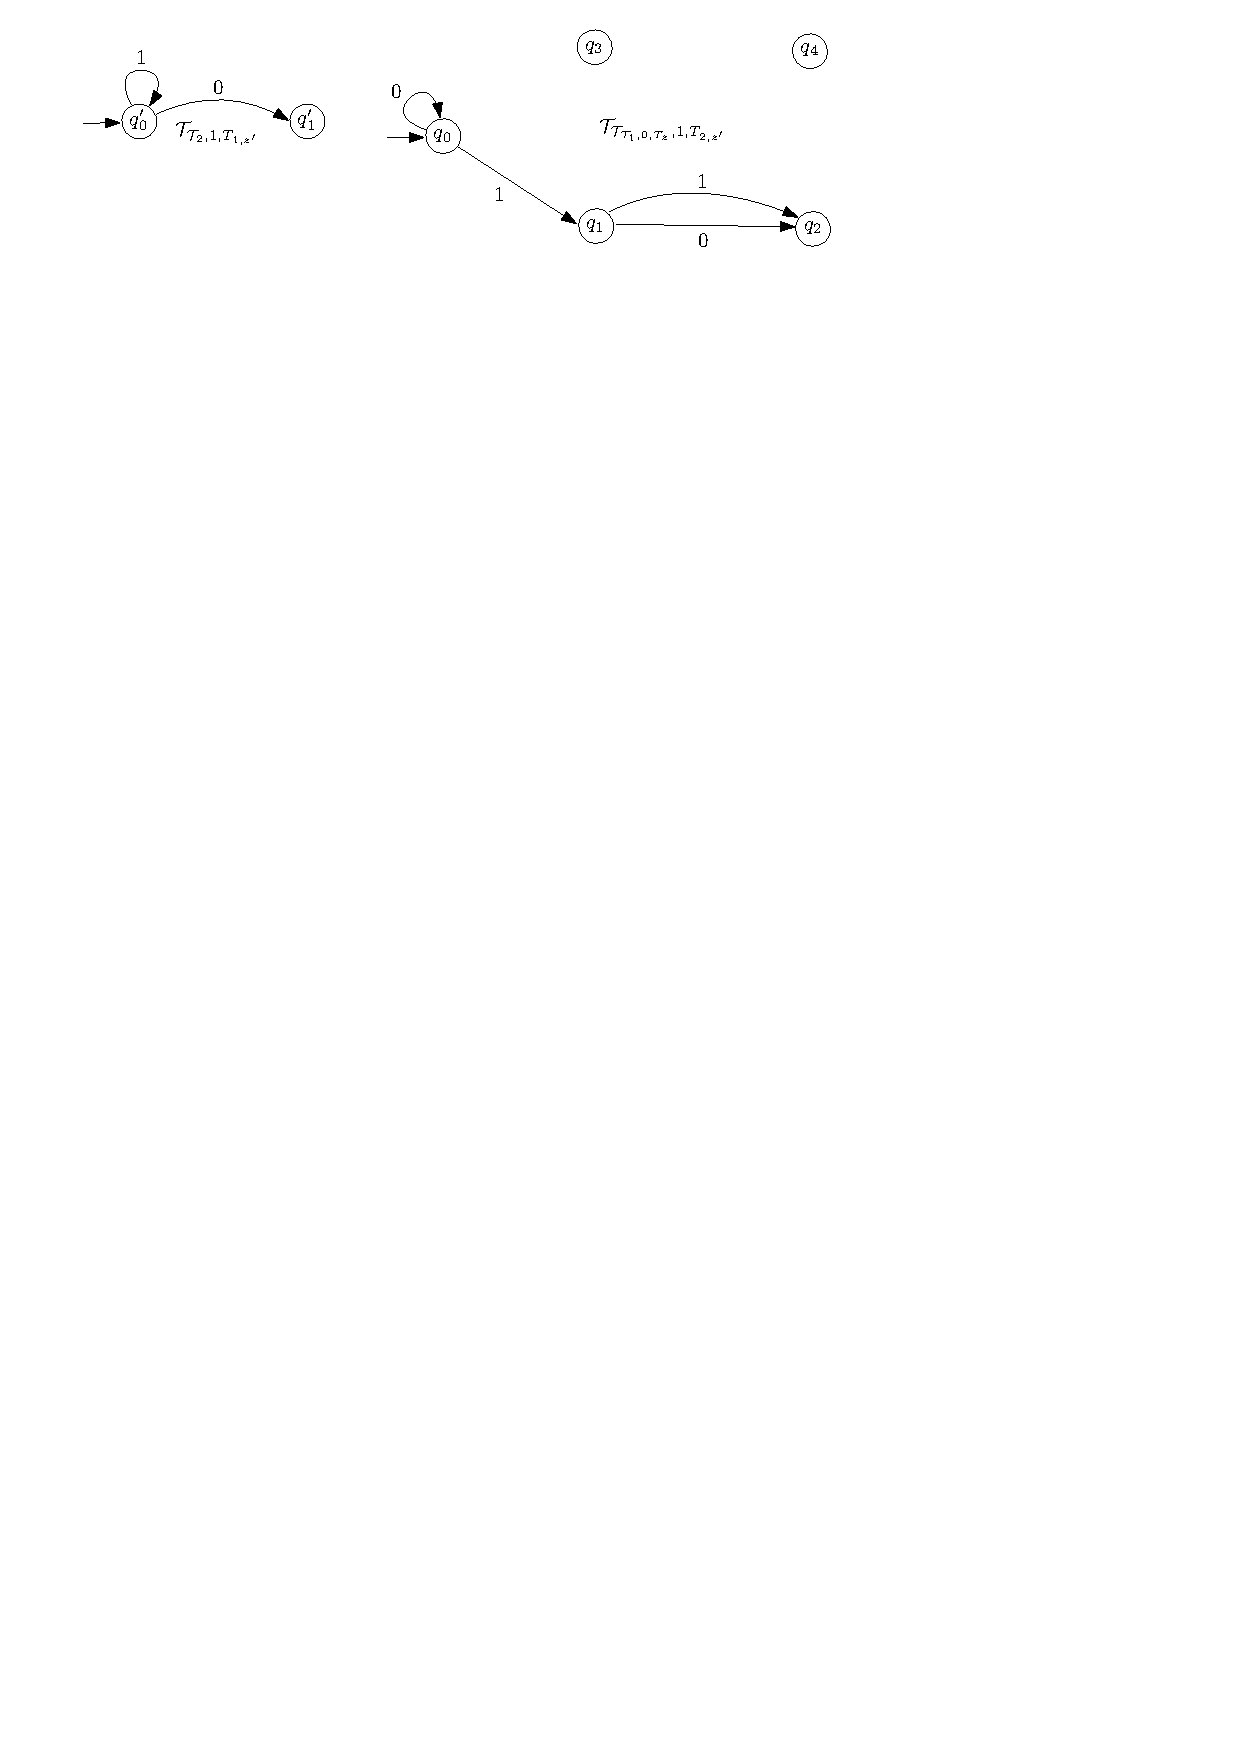
\includegraphics[scale=0.7]{single-letter-example-nested-2.pdf}
\end{center}
\caption{$\cT_{\cT_2, 1, T_{1,z'}}$ and $\cT_{\cT_{\cT_1, 0, T_z}, 1, T_{2,z'}}$}\label{fig-sl-exmp-nested-2}
\end{figure}
\end{example}




\subsubsection{Complexity}

To show that the aforementioned nondeterministic decision procedure works in exponential space, it is sufficient to show that the cardinalities of the sets $\cE(x)$ are exponential w.r.t. the size of $C$.

\begin{proposition}\label{prop-sl-comp}
The cardinalities of $\cE(x)$ for the variables $x$ in $G_C$ are at most exponential in $\dmdidx(G_C)$, the diamond index of $G_C$.
\end{proposition}
Therefore, according to Proposition~\ref{prop-sl-comp}, if the diamond index of $G_C$ is bounded by a constant $c$, then the cardinalities of $\cE(x)$ become \emph{polynomial} in the size of $C$ and we obtain a polynomial space decision procedure. In this case, we conclude that the satisfiability problem is PSPACE-complete.

\begin{proof}[Proof of Proposition~\ref{prop-sl-comp}]
Let $K$ be the maximum of $|\cE_0(x)|$ for $x \in \vars(\varphi)$. 

For each variable $x$ in $G_C$, all the regular constraints in $\cE(x)$ are either from $\cE_0(x)$, or are generated from some regular constraints from $\cE_0(x')$ for the ancestors $x'$ of $x$. Let $x'$ be an ancestor of $x$. Then for each $(\cT, \cP) \in \cE_0(x')$, according to Step I in the decision procedure, by an induction on the maximum length of the paths in from $x'$ to $x$, we can show that the number of elements in $\cE(x)$ that are generated from $(\cT, \cP)$ is at most the number of different paths from $x'$ to $x$. 
%
From Proposition~\ref{prop-di}, we know that there are at most $(|\vars(\varphi)||E_C|)^{O(\dmdidx(G_C))}$ different paths from $x'$ to $x$. Since there are at most $|\vars(\varphi)|$ ancestors of $x$, we deduce that $|\cE(x)| \le |\vars(\varphi)|\ K\ (|\vars(\varphi)||E_C|)^{O(\dmdidx(G_C))}$.
\end{proof}

%%%%%%%%%%%%%%%%%%%%%%%%the original complexity analysis%%%%%%%%%%%%%%%%%%%%%%%%
%%%%%%%%%%%%%%%%%%%%%%%%the original complexity analysis%%%%%%%%%%%%%%%%%%%%%%%%
%%%%%%%%%%%%%%%%%%%%%%%%the original complexity analysis%%%%%%%%%%%%%%%%%%%%%%%%
%
\hide{
\begin{proposition}
The cardinalities of $\cE(x)$ for the variables $x$ in $G_C$ are at most exponential  in the size of $C$ and become polynomial for $\strline_{\sf ss}[\replaceall]$ formulae.
\end{proposition}

\begin{proof}
%The transition graphs $\cT=(Q, \delta)$ and $\cT'=(Q', \delta')$ are said to be \emph{isomorphic} if there is a bijection $\pi: Q \rightarrow Q'$ such that for each $q, q' \in Q$ and $a \in \Sigma$, $(q, a, q') \in \delta$ iff $(\pi(q), a, \pi(q')) \in \delta'$.
%
Let $K$ denote the maximum cardinality of $\cE_0(x)$ for vertices $x$ in $G_C$.
%In addition, for each node $x$ in $G_C$, let $\#^{\sf anc}$
%In addition, let $M$ denote the maximum size (number of states) of the NFA in $\cE_0(x)$ for nodes $x$ in $G_C$.
For each $i$ and each vertex $x$ in $G_C$, let  $\#^{\sf anc}_i(x)$ denote the number of ancestors of $x$ in $G_i$.
%, in addition, let ${\sf Idx}^{\sf arb}_i(x)$ denote the maximum number of join vertices in a path starting from $x$ in $G_i$.

%the number of edges of $G_0 \setminus G_i$ (i.e. the subgraph of $G_0$ comprising all the edges not in $G_i$) that are co-reachable from $x$ in  $G_0 \setminus G_i$.

% and $\#_{\sf lft}(x)$ denote the number of $\rpleft$-edges that are co-reachable from $x$ in $G_C$.

%Then the proposition follows from the following claim, since for each node $x$, $|\cE(x)| \le |\cG(\cE(x))|M^2$.

We first prove the following claim.

\smallskip

\noindent {\bf Claim}. For each $i$ and each vertex $x$ in $G_C$,
$|\cE_i(x)| \le 3^i K$. In addition, if $C \in \strline_{\sf ss}[\replaceall]$, then for each non-source variable $x$ in $G_C$, $|\cE_i(x)| \le (\#^{\sf anc}_0(x)-\#^{\sf anc}_i(x)+1) K$.
%In addition, if $G_C$ is a tree, then $|\cE_i(x)| \le (\#^{\sf anc}_0(x)-\#^{\sf anc}_i(x)+1) K$.

\smallskip

We prove the claim by an induction on $i$.

\smallskip


\noindent {\it Induction base}: $i=0$. Evidently $|\cE_0(x)| \le K = 3^0 K$. Moreover, if $C \in \strline_{\sf ss}[\replaceall]$, then for each non-source variable $x$, $|\cE_0(x)| \le K = (\#^{\sf anc}_0(x)-\#^{\sf anc}_0(x)+1) K$.
% = (\#^{\sf anc}_0(x)-\#^{\sf anc}_0(x)+1) K$.

\smallskip

\noindent {\it Induction step}:
Suppose $i > 0$.

Let $x$ be the vertex without predecessors and with successors in $G_{i-1}$ that is used to construct $G_{i}$. In addition, let $(x, (\rpleft, a), y)$ and $(x, (\rpright, a), z)$ be the two edges out of $x$ in $G_{i-1}$.

Let us first assume $y \neq z$.
Then $|\cE_{i}(z)| \le |\cE_{i-1}(z)| + |\cE_{i-1}(x)|$ and $|\cE_{i}(y)| \le |\cE_{i-1}(y)| + |\cE_{i-1}(x)|$.  By the induction hypothesis, $|\cE_{i-1}(x)| \le  3^{i-1} K$, $|\cE_{i-1}(y)| \le 3^{i-1} K$, and $|\cE_{i-1}(z)| \le 3^{i-1} K$. Therefore, $|\cE_{i}(z)|  \le |\cE_{i-1}(z)| + |\cE_{i-1}(x)| \le 3^{i-1} K + 3^{i-1} K \le 3^i K$. Similarly, $|\cE_{i}(y)| \le 3^i K$.

Next, we assume $y = z$. Then $|\cE_{i}(z)| \le |\cE_{i-1}(z)| + |\cE_{i-1}(x)| + |\cE_{i-1}(x)| \le 3* 3^{i-1} K = 3^i K$.

Let us assume that $C \in \strline_{\sf ss}[\replaceall]$, moreover, either $y$ or $z$ is not a source variable. Then $y \neq z$. Because otherwise, the in-degree of $y=z$ in $G_C$ is more than one, from the fact that $G_C$ is source-sharing, we deduce that $y=z$ has to be a source variable, a contradiction. Let us first assume that $z$ is not a source variable. Then the in-degree of $z$ is one, that is, the edge from $x$ to $z$ is the only incoming edge of $z$ in $G_C$. From this, we deduce that  $\cE_{i-1}(z) = \cE_0(z)$. Therefore, $|\cE_{i}(z)| \le |\cE_{i-1}(z)| + |\cE_{i-1}(x)| \le K + |\cE_{i-1}(x)|$. By the induction hypothesis, $|\cE_{i-1}(x)| \le (\#^{\sf anc}_{0}(x) - \#^{\sf anc}_{i-1}(x)+1)K$. We deduce that $|\cE_{i}(z)| \le K+ (\#^{\sf anc}_{0}(x) - \#^{\sf anc}_{i-1}(x)+1)K$. Moreover, since $\#^{\sf anc}_{0}(z) = \#^{\sf anc}_{0}(x)+1$ and $\#^{\sf anc}_{i-1}(x)=\#^{\sf anc}_{i}(x)= \#^{\sf anc}_{i}(z)=0$, we have $|\cE_{i}(z)| \le K+ (\#^{\sf anc}_{0}(z)-1 - \#^{\sf anc}_{i}(z)+1)K = (\#^{\sf anc}_{0}(z) - \#^{\sf anc}_{i}(z)+1)K$.
Similarly, if $y$ is not a source variable, we have $|\cE_{i}(y)| \le |\cE_{i-1}(y)| + |\cE_{i-1}(x)| = |\cE_{0}(y)| + |\cE_{i-1}(x)| \le K+|\cE_{i-1}(x)| \le K+ (\#^{\sf anc}_{0}(x) - \#^{\sf anc}_{i-1}(x)+1)K \le K+ (\#^{\sf anc}_{0}(y)-1 - \#^{\sf anc}_{i}(y)+1)K = (\#^{\sf anc}_{0}(y) - \#^{\sf anc}_{i}(y)+1)K$.

The proof of the claim is complete.

To complete the proof of the proposition, let $H$ be the maximum length of the paths in $G_C$. From the claim, we deduce that for each non-source variable $x$, $|\cE(x)| \le (H-1)K$. In addition, for each source variable $y$ in $G_C$, suppose that the in-degree of $y$ in $G_C$ is $m$, then $|\cE(y)| \le K + \sum \limits_{x: \mbox{ \small predecessor of } y} |\cE(x)| \le  K+m(H-1)K=(mH-m+1) K$.
%
Therefore, we conclude that if $C \in \strline_{\sf ss}[\replaceall]$, then the cardinalities of $\cE(x)$ become polynomial in the size of $C$.
\end{proof}
}
%%%%%%%%%%%%%%%%%%%%%%%%%%%%%%%%%%%%%%%%%%%%%%%%%%%%%%%%%%%%%%
%%%%%%%%%%%%%%%%%%%%%%%%%%%%%%%%%%%%%%%%%%%%%%%%%%%%%%%%%%%%%%
%%%%%%%%%%%%%%%%%%%%%%%%%%%%%%%%%%%%%%%%%%%%%%%%%%%%%%%%%%%%%%

%\begin{quote}
%\it Let $x$ be a node in the graph without predecessors and $x = \replaceall(y, a, z)$ be a conjunct of $\varphi$ and $\cA_1, \dots, \cA_m$ be a collection of regular constraints for $x$. Then remove the two edges out of $x$, guess $T_{i, z} \subseteq Q_i \times Q_i$ for $i \in [m]$, and add additional regular constraints to $y$ and $z$ as specified above.
%\end{quote}

%For doing this, we need deal with the typical situation that $x = \replaceall(y, a, z)$  and the regular constraints for $x$ are specified by

%We first introduce a concept of dependency graphs.


